\newpage
\subsection{Sinus, Cosinus und Tangens}

\hfill \break
Der Einheitskreis ist ein Kreis mir einem Radius von der Länge 1. Es wird keine Einheit angegeben.

\hfill \break
\begin{itemize}
    \item $Sin(\alpha) = \frac{\textcolor{red}{3}}{\textcolor{purple}{5}} = \frac{\textcolor{cyan}{6}}{\textcolor{violet}{7.5}}= \frac{\textcolor{cyan}{Gegenkatete}}{\textcolor{violet}{Hypothenuse}}$
    \item $Cos(\alpha) = \frac{\textcolor{green}{4}}{\textcolor{purple}{5}} = \frac{\textcolor{olive}{8}}{\textcolor{violet}{7.5}}= \frac{\textcolor{olive}{Ankatete}}{\textcolor{violet}{Hypothenuse}}$
    \item $Tan(\alpha) = \frac{\textcolor{red}{3}}{\textcolor{green}{4}} = \frac{\textcolor{cyan}{6}}{\textcolor{olive}{8}} = \frac{\textcolor{cyan}{Gegenkatete}}{\textcolor{olive}{Ankatete}}$
\end{itemize}


\hfill \break
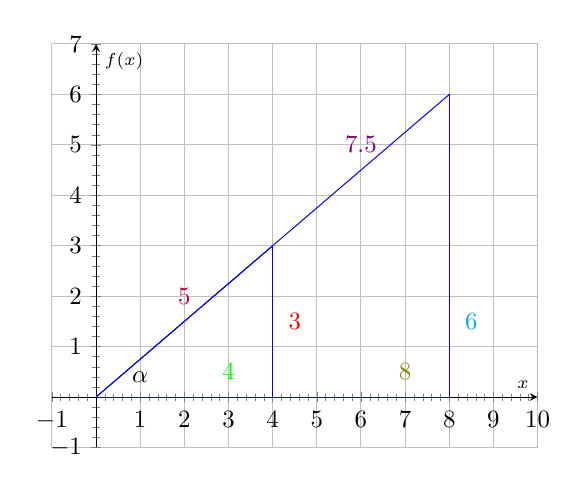
\begin{tikzpicture}[scale=0.9]
    \begin{axis}%
        [
            grid=major,
            xtick={-1,0,...,10},
            minor x tick num=4, % 4 minor ticks => 5 subintervals
            xmin=-1,
            xmax=10,
            xlabel={\scriptsize $x$},
            axis x line=middle,
            ytick={-1,0,...,7},
            minor y tick num=4,  % 4 minor ticks => 5 subintervals
            ymin=-1,
            ymax=7,
            ylabel={\scriptsize $f(x)$},
            axis y line=middle,
            no markers,
            samples=100,
            domain=-6:6,
        ]

        \draw[color=blue] (0,0) -- (8,6);
        \draw[color=blue] (0,0) -- (4,3);
        \draw[color=blue] (8,0) -- (8,6);
        \draw[color=blue] (4,0) -- (4,3);
        \draw[color=blue] (4,0) -- (0,0);
        \draw[color=blue] (8,0) -- (0,0);

        \node[color=black] at (1,0.4) {$\alpha$};

        \node[color=purple] at (2,2) {$5$};
        \node[color=violet] at (6,5) {$7.5$};
        \node[color=red] at (4.5,1.5) {$3$};
        \node[color=cyan] at (8.5,1.5) {$6$};
        \node[color=green] at (3,0.5) {$4$};
        \node[color=olive] at (7,0.5) {$8$};
    \end{axis}
\end{tikzpicture}


\hfill \break
Die Umkehrung vom Sinus ist der Arkussinus.


\hfill \break
Example zum errechnen von $\alpha$:\\
\fboxrule=0.8pt \fcolorbox{black}{lightgray}{%
    \begin{tabular}[t]{@{}l@{}}
        $Sin(\alpha) = 0.6$ // Te $\rightarrow$ $sin^{-1}$ \\
        $\alpha = 36.87^{\circ}$                           \\
        \\
        \\
        $Cos(\alpha) = 0.8$ // Te $\rightarrow$ $cos^{-1}$ \\
        $\alpha = 36.87^{\circ}$
    \end{tabular}}
